\RequirePackage[l2tabu, orthodox]{nag}
\documentclass[12pt,chapterprefix=true,toc=bibliography,numbers=noendperiod,
               footnotes=multiple,twoside]{scrreprt}
\usepackage{fixltx2e} % LaTeX patches, \textsubscript
\usepackage{microtype}
\usepackage{cmap} % fix search and cut-and-paste in Acrobat
\usepackage{ifthen}
\usepackage[oldstylenums,largesmallcaps,easyscsl]{kpfonts}
\usepackage[T1]{fontenc}
\usepackage[utf8]{inputenc}
\usepackage[british]{babel}
\usepackage[table,hyperref,dvipsnames]{xcolor}
\usepackage{floatrow}
\usepackage{csquotes}
\usepackage{tabularx}
\usepackage{graphicx}
\usepackage{pdfpages}
\usepackage{multirow}
\usepackage{booktabs}
\usepackage{ctable}
\usepackage{algorithmicx}
\usepackage{algpseudocode}
\usepackage{attrib}
\usepackage{algorithm}
\usepackage{mathtools}
\usepackage[binary-units]{siunitx}
\usepackage[chapter]{minted}
\usepackage[font=small,labelfont=bf,format=plain]{caption}
\usepackage{subcaption}
\usepackage{paralist}
\usepackage[autocite=footnote,citestyle=authoryear-comp,bibstyle=authoryear,
            dashed=false,isbn=false,doi=false,backend=biber]{biblatex}
\usepackage[bookmarks,hidelinks]{hyperref}
\usepackage[noabbrev]{cleveref}

% TODO: list of figures, algorithms, tables?
% TODO: custom cover page?

%%% Custom LaTeX preamble
% serif, non-bold headings:
\addtokomafont{chapter}{\mdseries}
\addtokomafont{disposition}{\rmfamily}
\addtokomafont{descriptionlabel}{\rmfamily}
\addtokomafont{pageheadfoot}{\itshape}
% section numbering up to subsection
\setcounter{secnumdepth}{2}
% hyperlinks
\urlstyle{same} % normal text font (alternatives: tt, rm, sf)
\hypersetup{
  pdftitle={Extending Raft with structured voting},
  pdfauthor={Leonhard Markert (lm510), Emmanuel College}
}
\addbibresource{Bibliography.bib}
\pagestyle{headings}

\usemintedstyle{tango}
\newminted{cpp}{fontfamily=jkptt, fontsize=\small}
\newminted{erlang}{fontfamily=jkptt, fontsize=\small}
\newmint{erlang}{fontfamily=jkptt}

\DeclareFloatVCode{ruleabove}%
    {{\color{black}\par\rule\hsize{0.75pt}\vskip4pt\par}}
\DeclareFloatVCode{rulebelow}%
    {{\color{black}\par\vspace{-20pt}\rule\hsize{0.75pt}\vskip10pt\par}}
\floatsetup[listing]{
    style=plain,
    frameset={\fboxsep6pt}
    capposition=bottom,
    precode=ruleabove,
    midcode=rulebelow
}

\DeclarePairedDelimiter{\oiv}{]}{[}

\sisetup{detect-all}

% source: http://la-tex.dreamwidth.org/3017.html
% This command computes and creates a vertical space
% depending on the number of rows to compensate for.
% It makes use of the counter verticalcompensationrows
% and the length \verticalcompensationlength which equals
% \aboverulesep plus \belowrulesep
\newlength{\verticalcompensationlength}
\setlength{\verticalcompensationlength}{\aboverulesep}
\addtolength{\verticalcompensationlength}{\belowrulesep}
\newcounter{verticalcompensationrows}
\newcommand{\verticalcompensation}[1]{%
\setcounter{verticalcompensationrows}{#1}%
\addtocounter{verticalcompensationrows}{-1}%
\vspace*{-\value{verticalcompensationrows}\verticalcompensationlength}%
}

% This command reimplements \multirow to compensate
% for the vertical offset, but looses some functionality
% of the \multirow command (not discussed here).
\newcommand{\multirowbt}[3]{%
\multirow{#1}{#2}{\verticalcompensation{#1}#3}%
}

\setlength{\bibitemsep}{.5\baselineskip}
% \setlength{\bibnamesep}{\baselineskip}

\hyphenation{com-po-nent}

% custom commands
\newcommand{\requestVoteRPC}[0]{\texttt{requestVote} \textsc{rpc}}
\newcommand{\appendEntriesRPC}[0]{\texttt{appendEntries} \textsc{rpc}}
\newcommand{\ECC}[0]{\textsc{ec}2 }

\newcommand{\zerospacing}[0]{\medmuskip=0mu}
\newcommand{\high}[0]{{\color{purple!90}\zerospacing \(\bullet \bullet \bullet\)} }
\newcommand{\hard}[0]{{\color{purple!90}\zerospacing \(\bullet \bullet \bullet\)} }
\newcommand{\medium}[0]{{\color{violet!80}\zerospacing \(\bullet \bullet\)} }
\newcommand{\easy}[0]{{\color{teal!80}\(\bullet\)} }
\newcommand{\low}[0]{{\color{teal!80}\(\bullet\)} }

\newcommand{\yes}{{\fontfamily{jkposn}\selectfont\textsc{Yes}}}
\newcommand{\no}{{\fontfamily{jkposn}\selectfont\textsc{No}}}

\newlength{\smallbaselineskip}
\setlength{\smallbaselineskip}{13.6pt}

%%% Body
\begin{document}

%TC:ignore

% \frontmatter
\pagenumbering{roman}

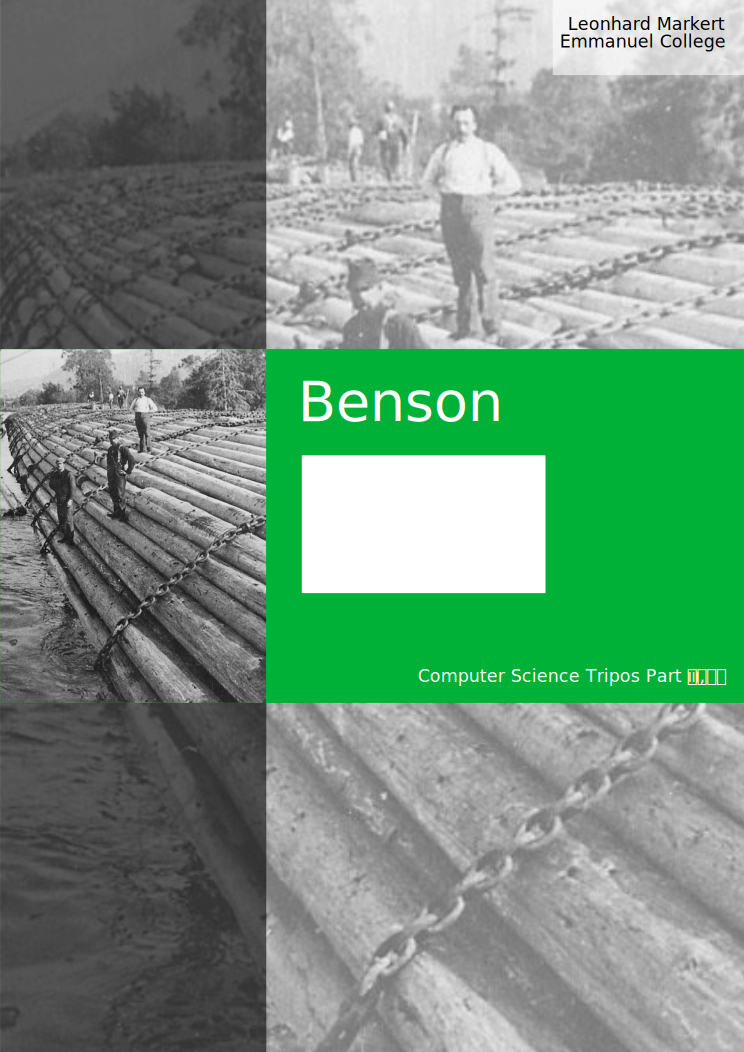
\includepdf{Cover.pdf}



\chapter*{Proforma}
\label{ch:proforma}

\begin{center}
{\renewcommand{\arraystretch}{1.5}%
\begin{tabularx}{330pt}{rX}
\textbf{Name and College} & Leonhard Markert, Emmanuel College \\
\textbf{Project Title} & Extending Raft with structured voting \\
\textbf{Examination} & Computer Science Tripos, Part \textsc{ii}, June 2014 \\
\textbf{Word Count} & XXX words \\
\textbf{Project Originator} & Leonhard Markert \\
\textbf{Project Supervisors} & Malte Schwarzkopf and Ionel Gog
\end{tabularx}}
\end{center}

\section*{Original aims of the project}
\label{sc:original-aims}

Extending Rafter,\footnote{Rafter is an open source project hosted on GitHub (\url{http://github.com/andrewjstone/rafter}).} an implementation of the new Raft \autocite{raft} consensus algorithm written in Erlang, with the ability to form quorums using structured voting schemes. This includes implementing and testing voting structure generators for at least the Majority Protocol and the Grid Protocol. In order to compare the performance of my voting algorithms with those used in the original Rafter code, and to measure how different structured voting schemes scale with the number of nodes, benchmarks need to be run with a Rafter cluster in the Amazon Elastic Compute Cloud.

\section*{Work completed}
\label{sc:work-completed}

All objectives outlined in the proposal have been met: I have written a structured voting scheme module for Rafter, and implemented voting structure generators for the Majority Protocol and the Grid Protocol. As an extension to the original aims of the project, a voting structure generator for the Tree Quorum Protocol has been implemented. Benchmarks in the Amazon cloud have been run, and the results have been analysed and evaluated.

\section*{Special Difficulties}
\label{sc:special-difficulties}

None.

\newpage

\section*{Declaration of Originality}
\label{sc:declaration-of-originality}

I, Leonhard Markert of Emmanuel College, being a candidate for Part~\textsc{ii} of the Computer Science Tripos, hereby declare that this dissertation and the work described in it are my own work, unaided except as may be specified below, and that the dissertation does not contain material that has already been used to any substantial extent for a comparable purpose.

\vspace{0.3in}
Signed

\vspace{0.2in}
Date \hspace{0.4in} \today



\chapter*{Acknowledgements}
\label{ch:acknowledgements}

\begin{itemize}
    \item Malte Schwarzkopf and Ionel Gog
    \item Christian Storm
    \item Andrew Stone
\end{itemize}

\tableofcontents

% \mainmatter

%TC:endignore



\chapter{Introduction}
\label{ch:introduction}

\pagenumbering{arabic}

This dissertation describes how I extended an implementation of the new Raft consensus algorithm with the ability to form quorums using structured voting schemes.

% \begin{itemize}
    % \item Principal motivation for the project
    % \item How the work fits into the broad area of surrounding CS
    % \item Survey of related work
% \end{itemize}

% \begin{itemize}
    % \item Raft: consensus protocol, asymmetric: leader, follower, candidate -- elections, majority voting by default; state machine, backend, ``understandable'' Paxos replacement -- strongly consistent (all operations are seen in the same order by all nodes); correctness proof \parencite{raft} \parencite{raftproof}
    % \item Structured voting: more efficient / available (less cost), example: Grid protocol, key insight: don't need majority to guarantee mutual exclusion; tree-shaped voting structures: generalised framework; logical structure on nodes; smaller quorums
    % \item Motivation: combine Raft and structured voting (\textit{write} quorums specifically)
    % \item Failure model: no Byzantine failures -- servers either work or not; fail-stop, permanent/volatile memory, lost/delayed messages but not corrupted
% \end{itemize}

\section{Motivation}
\label{sc:motivation}

As ever-increasing amounts of data are being handled in commercial settings as well as in research, distributed systems for data processing and storage are becoming increasingly ubiquitous. This development brings about the need to increase fault tolerance in the face of arbitrary network and node failures.

According to Eric Brewer's famous \textsc{cap} theorem \autocite{cap}, a partition tolerant system cannot be both strictly consistent and maximally available.\footnote{The terms consistency, availability and partition tolerance are defined in \cref{ssc:cap-acid-and-base}.} Many recent distributed data stores sacrifice consistency for availability. Some applications, however, require strong consistency guarantees -- data backup and configuration management systems, for example. Consensus protocols like Paxos \autocite{paxos} and Raft \autocite{raft} guarantee consistency at the cost of decreased availability.

Today's popular distributed data stores use \emph{unstructured} voting schemes. This means that in order for an operation to proceed, a certain number of processes must agree to it. Majority voting is a widely used instance of an unstructured voting scheme, requiring the consensus of a majority of the processes in the cluster. Some systems, notably Dynamo \autocite{dynamo} and the more recent Cassandra \autocite{cassandra}, allow quorums to be smaller than necessary to guarantee consistency. This gives rise to a less well-defined notion of \enquote{eventual consistency}, and enables the system administrator to trade decreased consistency for increased availability.

\emph{Structured} voting schemes, on the other hand, impose a logical structure of some kind onto the cluster. They are strongly consistent by default, and take the identity of each process into account when forming quorums, instead of merely counting them (as unstructured voting schemes do). This allows for much more detailed tuning of the system's availability as the structure of the cluster and the properties of individual nodes can guide the selection and configuration of the structured voting scheme.

In this project, I added support for structured voting schemes to an existing implementation of Raft. My aim was to allow more fine-grained availability and scalability trade-offs for data storage systems built on top of this implementation while still providing the same consistency guarantees as the original Raft algorithm.

% Regarding availability, structured voting schemes are more flexible than unstructured voting schemes like the Majority Protocol, and can in some cases be tailored to resist certain failure modes. Concerning scalability, the number of nodes involved in an election is always \(O(n)\) for any reasonable unstructured voting scheme. Structured voting schemes, on the other hand, can allow for elections with fewer nodes.

\section{Challenges}
\label{sc:challenges}

So far, structured voting schemes have mostly been confined to academic papers and theoretical analysis. I am not aware of any popular modern distributed storage system that uses structured voting schemes to generate quorums. Since the discovery of a unified framework for specifying structured voting schemes by \citeauthor{generators},\autocite{generators} it has become possible to implement a generic voting structure interpreter that works with any voting structure specified in this way. This allows distributed systems to switch between different voting schemes without having to re-implement the code which decides whether or not a given set of nodes constitutes a quorum.

Due to the lack of previous implementations of structured voting scheme algorithms, I had to design my own, based on the high-level description from Storm's PhD thesis.\autocite{voting}

In addition, distributed programming in itself is a challenge: any component may fail at the least convenient time; network connections may be unreliable; messages may be dropped, duplicated or reordered. Fortunately, the programming language Erlang\footnote{\url{http://www.erlang.org}} used in this project provides some tools that make writing distributed systems a bit easier.

Lastly, benchmarking a distributed system running in the cloud is difficult. Thorough planning and a high degree of automation is required to make it at all feasible.

\section{Related work}
\label{sc:related-work}

The primary source of ideas for this project was Christian Storm's PhD thesis, \citetitle{voting} \parencite{voting}, which puts unstructured and structured voting schemes into a common framework and analyses them using Petri nets.

Literature on voting schemes goes back much further: Majority voting \autocite{majority} was introduced in \citedate{majority}; the Tree Quorum Protocol \autocites{tree}{gen-tree} and the Grid Protocol \autocites{grid}{bettergrid} were invented in the early 1990s.

The Raft consensus algorithm, on the other hand, is a very recent addition to distributed systems toolset. Indeed, at the time of this writing, the original Raft paper is still a draft \autocite{raft}. It has nonetheless led to a lot of excitement since its first version, and a few dozen implementations in different languages and in various stages of development exist.

Considering the environment in which distributed systems run, many big internet firms have been operating data centres for years now. This has enabled them to collect data about the frequency of different types of failures over time. I used data compiled by Google Senior Fellow Jeff Dean to direct my failure simulation. \autocite{distr}

During an internship at \textsc{tng} Technology Consulting\footnote{\url{http://www.tngtech.com}}, I produced a working prototype of a key-value store based on structured voting schemes using the Node.js JavaScript framework.\footnote{Node.js (\url{http://nodejs.org}) is a platform for building network applications in JavaScript.} This was done under the supervision of Christoph Stock and Christian Storm.



\chapter{Preparation}
\label{ch:preparation}

A lot of reading and careful planning was necessary before I could start extending Rafter with structured voting. I first needed to understand \citeauthor{generators}'s unified framework for specifying voting structures, primarily by reading \citeauthor{voting}'s PhD thesis \autocite{voting}. I had to familiarise myself with Rafter and the programming language it is written in, Erlang; and finally, I had to set up a benchmarking environment in Amazon's Elastic Compute Cloud.

In this chapter, I will first introduce some of the challenges posed by distributed systems in general. I will give an overview of the Raft consensus algorithm, and then describe structured voting schemes, taking the Grid Protocol as an example. I will mention the software engineering techniques that were applied to the project. Finally, a list of the languages, tools and libraries used in this project as well as a short description of my development environment an backup strategy will be given.

% \begin{itemize}
    % \item Work undertaken before code was written
    % \item Refinement of project proposal
    % \item Professional approach: Requirements analysis!, reference Software Engineering techniques
    % \item PLs and systems which had to be learnt, theories and algorithms which required understanding
% \end{itemize}

\section[Introduction to distributed systems]{Introduction to distributed systems: \textsc{cap}, \textsc{acid} and \textsc{base}}
\label{ssc:cap-acid-and-base}

Eric Brewer's famous \textsc{cap} theorem states that any distributed system can provide at most two out of the three desirable properties consistency (\textsc{c}), availability (\textsc{a}), and partition tolerance (\textsc{p}).\autocite{cap} The following definitions are adapted from the proof of the \textsc{cap} theorem by \citeauthor{capproof}:\autocite{capproof}

\begin{description}
    \item[Consistency] There must exist a total order on all operations such that each operation looks as if it were completed at a single instant. An important consequence of this \emph{linearisable} (or \emph{atomic}) consistency guarantee is that any read operation that begins after a write operation completes must return that value, or the result of a later write operation.\footnote{As \textcite{capproof} point out, the term \emph{consistency} is highly overloaded. The reader may observe that the notion of atomic consistency used in this dissertation subsumes what is called atomicity and consistency in the context of \textsc{acid} (\enquote{atomic, consistent, isolated, durable}) databases.}
    \item[Availability] Every request received by a non-failing node in the system must result in a response.
    \item[Partition tolerance] The system continues to operate despite arbitrary message loss. This includes network partitions, where all messages sent from nodes in one component of the partition to nodes in another component are lost.
\end{description}

Out of those three, partition tolerance is required in almost all cases. As \citeauthor{needp} puts it in his article \citetitle{needp}:

\begin{quote}
    For a distributed \dots{} system to \emph{not} require partition tolerance it would have to run on a network which is guaranteed to never drop messages \dots{} and whose nodes are guaranteed to never [fail]. [These] types of systems \dots{} don't exist.
    \attrib{\cite{needp}}
\end{quote}

This leaves designers of distributed systems with the task of finding the right trade-off between consistency and availability, both of which should be considered as continuous rather than binary properties \autocite{cap12}. With the rise of commercial databases of unprecedented scale over the last decade, consistency (in its strict form as defined above) is in many cases sacrificed for increased availability.%
\footnote{This has been heralded as a paradigm shift from the \textsc{acid} to the \textsc{base} (\enquote{basically available, soft state, eventually consistent}) model \parencite{base}.} %
The authors of \citetitle{dynamo} describe this as follows:%
\footnote{Notable other eventually consistent systems include Cassandra \parentext{\citeurl{cassandra}}, Riak \parentext{\citeurl{riak}} and HBase \parentext{\citeurl{hbase}}.}

\begin{quote}
    For systems prone to server and network failures, availability can be increased by using optimistic replication techniques, where \ldots{} concurrent, disconnected work is tolerated. The challenge with this approach is that it can lead to \emph{conflicting changes which must be detected and resolved}.
    \attrib{\cite{dynamo}}
\end{quote}

The conflict detection and resolution mechanisms required by applications built on top of eventually consistent systems increase their complexity compared to those based on consistent systems, which do not need them. This begs the question: are there techniques that could be used to improve availability without giving up on consistency, allowing for simpler systems? The \textsc{cap} theorem tells us that we can never build strictly consistent and maximally available systems, but a different trade-off might be possible.

\section{Introduction to the Raft consensus algorithm}
\label{ssc:raft-consensus-algorithm}

Although still a draft, the paper describing the new Raft consensus algorithm \autocite{raft} has become widely known very quickly; dozens of implementations in various languages and stages of development already exist.\footnote{See \url{http://raftconsensus.github.io/\#implementations} for a list of Raft implementations.}

In the following, I will give a short overview of the Raft consensus algorithm. It is meant to introduce the terminology required for the Implementation and Evaluation chapters.

At its core, Raft uses a replicated state machine architecture, implemented using a replicated log (see \cref{fig:replicated-state-machine}): each log contains the same commands in the same order, so each state machine processes the same sequence of commands. Since the state machines are assumed to be deterministic, each computes the same state and the same sequence of outputs.

\begin{figure}[h]
    \centering
    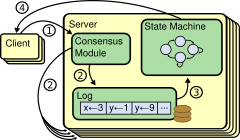
\includegraphics[width=0.5\textwidth, keepaspectratio]{Images/Replicated_state_machine.pdf}
    \caption{Replicated state machine architecture.
        \protect\attrib{\cite[2]{raft}}
    }
    \label{fig:replicated-state-machine}
\end{figure}

Raft implements this replicated log architecture using a collections of servers (a cluster) communicating via remote procedure calls (\textsc{rpc}s), of which there are two: \texttt{appendEntries} and \texttt{requestVote}. At any given time each server is either a \emph{leader}, \emph{follower}, or \emph{candidate} (see \cref{fig:consensus-fsm}). In normal operation, there is exactly one leader and all other servers are followers.

This requirement for each server to be in a specific state at any time makes it an \emph{asymmetric} consensus algorithm, as opposed to Paxos, which is \emph{symmetric} since it has no concept of \enquote{roles}. The designers of Raft made a conscious decision to build an asymmetric voting algorithm since it suits their philosophy of decomposition well:

\begin{quote}
    Raft implements consensus by first electing a distinguished leader, then giving the leader complete responsibility for managing the replicated log.
    \attrib{\cite[3]{raft}}
\end{quote}

\begin{figure}[h]
    \centering
    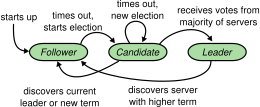
\includegraphics[width=0.5\textwidth, keepaspectratio]{Images/Consensus_FSM.pdf}
    \caption{Server states and the transitions between them.
        \protect\attrib{\cite[5]{raft}}
    }
    \label{fig:consensus-fsm}
\end{figure}

\minisec{Leader election}

A server remains in follower state as long as it receives valid heartbeats from a leader or candidate. If a follower receives no communication over a period of time, it assumes that there is no viable leader and begins an election to choose a new one. To do so, it transitions to \textit{candidate} state and issues \requestVoteRPC s in parallel to all other servers in the cluster. Then one of three things happens: (a) the candidate wins the election, (b) another server establishes itself as leader, or (c) a period of time goes by without a winner, in which case a new election is started.

Each server receiving a \requestVoteRPC{} will vote for at most one candidate, on a first-come-first-served basis. Once a candidate wins an election, it becomes the new leader and sends heartbeat messages to every other server to establish its authority.

\minisec{Log replication}

Each client request to a leader contains a command to be executed by the replicated state machines. The leader appends the command to its log as a new entry, then issues \appendEntriesRPC s in parallel to all other servers to replicate the entry. When the entry has been safely replicated, the leader applies the entry to its state machine and returns the result of that execution to the client (for a complete description of what it means for an entry to be \enquote{safely replicated}, \cite[see][subsection 5.3]{raft}.)

\minisec{Safety guarantees}

In order to guarantee overall correctness, different components of Raft are designed to make sure certain well-defined safety properties are true at all times (see \cref{sc:rafter-safety} for the complete list.) These properties are shown to hold and then used to prove correctness in the separate correctness proof \autocite{raftproof}.

Since my project involved changing the way in which quorums\footnote{A \emph{quorum} is a minimal subset of the cluster that an operation has to obtain \yes{} votes from in order to be performed. Majority voting, for example, specifies that any set of servers containing at least half the servers in the entire cluster constitutes a quorum.} are constructed, I had to pay special attention to the Election Safety property (stating that there can be at most one leader at any given time) and all the steps in the proof to do with quorums, in order to make sure all the desired properties still hold (see \cref{sc:rafter-proof} for a justification.)

\section{Introduction to structured voting schemes}
\label{ssc:structured-voting-schemes}

Voting schemes specify quorums. On an abstract level, they provide a procedure, which, given some knowledge about the entire cluster, decides whether or not a set of processes constitutes a quorum.

The Majority Protocol and Read One Write All are examples of unstructured voting schemes: whether or not a set of nodes forms a quorum depends only on its cardinality. In the case of the Majority Protocol, both read and write operations need the consent of a majority of processes; Read One Write All requires all processes to agree on write operations, whereas any one process can serve a read request.

By taking into account the identity of nodes (as opposed to just counting them), and superimposing a logical structure on the cluster, we can build \emph{structured} voting schemes.

\minisec{Quorum systems}

Formally, a quorum system is defined as a tuple of a read and a write quorum set whose elements are called read quorums and write quorums, respectively. These are constructed such that every write quorum intersects with every other write quorum and with every read quorum. Read quorums need not intersect pairwise \autocite{voting}.

The key realisation that lead to this project was that write quorums have precisely the property required for Raft's leader election, namely that any two write quorums intersect. From this point on, \emph{quorum} will mean \emph{write quorum} unless specifically noted otherwise.

\minisec{Structured voting by example}
\label{voting-example}

Structured voting schemes impose a logical structure on the set of processes and use structural properties to specify quorum systems. For example, the Grid Protocol arranges processes in a logical rectangular grid \autocite{grid}. A write quorum consists of all processes from a complete column plus one process from each column.

\begin{figure}[h]
    \centering
    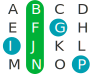
\includegraphics[scale=1]{Images/Grid_table.pdf}
    \caption[Grid protocol quorum table]{A Grid Protocol quorum: The entire second column (\texttt{B}, \texttt{F}, \texttt{J}, \texttt{N}) and one process from each other column (\texttt{I}, \texttt{G}, \texttt{P}) are included}
    \label{fig:grid-quorum}
\end{figure}

\minisec{Specifying voting structures}

\citeauthor{generators} present \emph{tree-shaped voting structures} as a universal quorum system representation in the form of semantics-enriched tree graphs. They are produced by voting structure-specific \emph{voting structure generators} \autocite{generators}.

In a tree-shaped voting structure, each node without children (a \emph{physical node}) represents a process. Nodes with children (called \emph{virtual nodes}) represent the structure of the voting scheme. The tree is to be interpreted such that votes flow upwards, from the physical nodes (the leaves of the tree) up to the virtual node at its root. \Cref{fig:grid4-state} on \cpageref{fig:grid4-state} illustrates this process for a Grid Protocol with four nodes. Examples of voting structures for different structured voting schemes are given in the Implementation chapter.

Note that in general, voting schemes are most naturally represented by directed acyclic graphs. But since from an algorithmic perspective tree structures are easier to operate on, the voting scheme graphs are simply transformed into trees by duplicating nodes as necessary, preserving correctness.

When a physical node casts its vote, its votes are added to the votes its parent virtual node has already received. If the sum of those votes equals or exceeds the parent node's threshold, then the parent node in turn passes its vote to its parent. An annotated example is given in \cref{fig:majority5-defs}.

\begin{figure}[h]
    \centering
    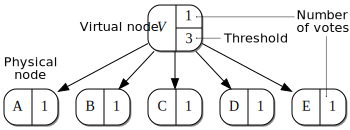
\includegraphics[scale=0.75]{Images/Majority5-defs.pdf}
    \caption[Tree-structured voting scheme for a Majority Protocol]{A tree-structured voting scheme for a Majority Protocol managing five processes. Three processes are enough to form a quorum, so the threshold of the root node is three.}
    \label{fig:majority5-defs}
\end{figure}

\section{Software engineering}
\label{sc:software-engineering}

An analysis of the requirements made the dependencies between the different components of the project explicit (see \cref{fig:dependencies}). This helped me draw up a development schedule, which is outlined in my proposal.

The main software engineering technique I used to increase my chances of success were \emph{modularisation} and \emph{testing} as explained below.

\subsection{Requirements analysis}
\label{sc:requirements-analysis}

The requirement for this project to be deemed a success was a demonstration of the extended version of Rafter running some application on a cluster in the Amazon Elastic Compute Cloud, using my structured voting modules to find quorums, and performing similarly to the original version of Rafter by Andrew Stone. \Cref{tab:objectives} gives a more detailed breakdown of the objectives, and \cref{fig:dependencies} shows the dependencies between the different components of the project.

\begin{table}[h]
    \centering
    \begin{tabularx}{\textwidth}{X c c}
        \toprule
        \textit{Objective} & \textit{Importance} & \textit{Difficulty} \\
        \midrule
        Voting structure and state type specification & \high & \medium \\
        Core voting algorithm & \high & \hard \\
        Voting structure visualiser & \medium & \medium \\
        Majority Protocol voting structure generator & \high & \easy \\
        Grid Protocol voting structure generator & \medium & \hard \\
        Tree Quorum Protocol voting structure generator & \low & \hard \\
        Rafter integration & \high & \hard \\
        Memcached frontend & \high & \medium \\
        Amazon \ECC benchmark set-up & \high & \medium \\
        Benchmarking and analysis of the results & \high & \medium \\
        \bottomrule
    \end{tabularx}
    \caption{Objectives of the project. \high high importance or hard; \medium medium importance or difficulty; \low low importance or easy.}
    \label{tab:objectives}
\end{table}

\begin{figure}[h]
    \centering
    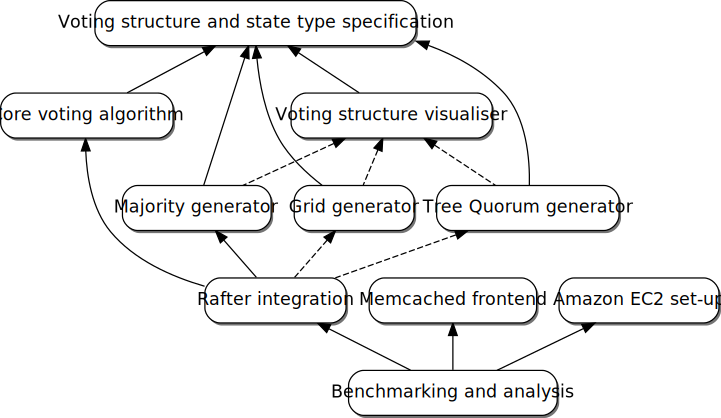
\includegraphics[width=1\textwidth, keepaspectratio]{Images/Dependencies.pdf}
    \caption{Dependency graph of the project's main components. Arrows point from dependent components to their dependencies. Dashed arrows indicate optional dependencies.}
    \label{fig:dependencies}
\end{figure}

\subsection{Modularisation}

This technique permeated all levels of the project. The code itself was written in a functional style, where each function typically spans between one and ten lines. This increased understandability by forcing me to split larger functions into smaller ones, each performing a small and well-defined task.

All development took place using Git, a popular version control system.\footnote{Git (\url{http://git-scm.com}) is an open source distributed version control system emphasising speed, originally developed by Linux Torvalds to simplify the development of the Linux kernel. Git supports very cheap and fast branching, a feature I used extensively in this project.} I used Git's branching facility to keep independent pieces of code separate during their development. Whenever code from different branches needed to be combined, I merged the required feature branches into a temporary branch. For convenience, all documentation (including the proposal, the progress presentation and this very dissertation) was kept under its own branch in the same repository.

\begin{table}[h]
    \centering
    \begin{tabularx}{\textwidth}{l X}
        \toprule
        \textit{Branch name} & \textit{Description} \\
        \midrule
        \texttt{structured-voting} & Voting algorithms and voting structure generators \\
        \texttt{memcached} & Memcached frontend \\
        \texttt{time-to-consensus} & Time-to-consensus logging \\
        \texttt{failure-command} & Follower failure simulation \\
        \texttt{ec2-integration} & Amazon \ECC instance administration scripts \\
        \bottomrule
    \end{tabularx}
    \caption{Feature branches used in the project repository}
    \label{tab:branches}
\end{table}

The voting algorithm, the voting structure visualiser and the generators for the Majority Protocol and the Grid Protocol were initially written and tested independently from Rafter. I integrate it with Rafter only once I was sufficiently confident in the correctness of the code. Thanks to the modularity of Rafter and the clear separation of concerns in my code, the integration process went through without major unexpected problems.

\section{Languages, tools and libraries}
\label{sc:tools}

In the inception phase of the project, I was faced with the decision of whether to use and existing implementation of Raft or write one from scratch. Since I was primarily interested in implementing structured voting algorithms and many implementations of Raft already exist, I decided to adapt an existing implementation.

Having written a distributed key-value store in Node.js during an internship, I decided to look for an implementation that used a programming language with built-in support for distributed programming that I had heard of, but never used before: Erlang. Out of the five Raft implementations written in Erlang, Andrew Stone's \emph{Rafter} seemed to be the most mature.\footnote{Rafter is an open source project hosted on GitHub (\url{http://github.com/andrewjstone/rafter}).}

\subsection{Structured voting extension}

The choice of Erlang and Rafter then determined my primary programming toolkit for the structured voting extension:

\begin{description}
    \item[Erlang] A dynamically typed functional programming language originally designed to run telephone switches, Erlang features a run-time system with built-in support for concurrency, distribution and fault tolerance.
        \attrib{\url{http://www.erlang.org}}
    \item[Open Telephony Platform] Commonly referred to as \enquote{the \textsc{otp}}, the Open Telephony Platform provides a set of Erlang libraries and design principles providing middle-ware to develop Erlang applications.
        \attrib{\url{http://www.erlang.org/doc}}
    \item[QuickCheck] A commercial testing framework for Erlang by Quviq \textsc{se}. Rafter's unit and integration tests use it, and I adapted and amended them to cover my code as well.
        \attrib{\url{http://www.quviq.com}}
    \item[Dialyzer] The \enquote{Discrepancy Analyzer for Erlang programs} is used to statically type-check Erlang programs.
        \attrib{\url{http://www.erlang.org/doc/man/dialyzer.html}}
\end{description}

\subsection{Benchmarking in the Amazon Elastic Compute Cloud}
\label{ssc:ec2-benchmarking}

In order to test and benchmark my code in a realistic environment, it needed to be run on a cluster of machines (as opposed to on a single computer) as this is how systems like Rafter are deployed in the real world. It was decided early on that I would run the project in the Amazon Elastic Compute Cloud (Amazon \textsc{ec2}). This allowed me to execute my benchmarks on up to twenty instances within the same data centre.

Orchestrating a cluster of Amazon \ECC instances and running benchmarks required its own set of tools.

\begin{description}
    \item[Fabric] is a Python library and command-line tool for streamlining the use of \textsc{ssh} for application deployment or systems administration tasks. Administrative functions like starting an Erlang node on an instance or compiling Rafter were defined as \emph{tasks} within the Fabric framework, which could then be executed on arbitrary \ECC instances with the help of the \enquote{awsfabrictasks} plugin.
        \attrib{\url{http://fabfile.org}, \url{https://awsfabrictasks.readthedocs.org}}
    \item[Boto] is a Python interface to Amazon Web Services, which includes the Elastic Compute Cloud. Awsfabrictasks is built on top of Boto, but I occasionally needed to use Boto's lower-level functionality directly.
        \attrib{\url{http://docs.pythonboto.org}}
    \item[Memaslap] was used to generate a test load on the cluster. It is part of libMemcached, an open source client library and toolset for the Memcached server. It is highly configurable, but still in an early phase of development, requiring me to patch its Makefile in order to get it to compile.
        \attrib{\url{http://libmemcached.org}}
\end{description}

\section{Development environment and backup}

The entire project was developed on my private laptop running Arch Linux, using the Vim text editor.\footnote{Vim is an extensible open source text editor for programmers. \url{http://www.vim.org}} I used version R16B03 of the Erlang interpreter and compiler. Apart from a few temporary files and compilation artefacts, every file I created was checked into some branch of the project's Git repository. See \cref{tab:branches} for a list of the main long-running branches created.

I used a public GitHub repository at \url{https://github.com/curiousleo/rafter} as a backup and a way to share files with my project supervisors; I pushed my changes to this repository after every significant change, but at least every few hours while I was working on the project. I took daily backups of my home directory, which contained the project repository, to an external hard drive.

\section{Summary}

In this chapter, I gave a brief introduction to distributed systems, precisely defining the terms consistency, availability and partition tolerance as they are understood in the context of the \textsc{cap} theorem. This was followed by an overview of the Raft consensus algorithm, where I explained the state machine approach to building distributed systems. Structured voting schemes were introduced by way of an example, namely the Grid Protocol. Tree-shaped voting structures were explained, and a labelled example was given for the Majority Protocol.

I listed this project's objectives, analysed the dependencies between its components, and elaborated on the role of modularisation and testing. Lastly, I talked about the programming languages and tools I used in this project and the development environment and backup strategy employed.



\chapter{Implementation}
\label{ch:implementation}

% \begin{itemize}
    % \item Describe what was actually produced
    % \item Design strategies (looking ahead to the testing stage)
    % \item Draw attention to the parts of the work which are not your own
    % \item Mention major milestones
% \end{itemize}

This chapter describes the implementation of the structured voting extension for Rafter and the benchmarking set-up.

The implementation phase of this project took place in two stages: At first, I concentrated on writing the structured voting code, which I subsequently integrated into Rafter.

In the second stage, I set up the benchmarking environment. This included adding logging facilities to Rafter, but also writing Fabric tasks to automate the actual benchmarking process in the Amazon Elastic Compute Cloud.

% also: how much of the code is mine? -- \texttt{git diff master --stat src/}

\section{Voting algorithm and data types}
\label{sc:voting-algo}

I started the implementation of the project by defining the data structures used to represent voting structures and voting states. These are passed around between different components, and designing them well was therefore a high priority.

The data structure representing a \emph{voting structure} has two components:

\begin{itemize}
    \item The voting structure itself. It is a tree whose nodes are annotated with the number of votes and, in the case of virtual nodes, the threshold (see \cref{fig:majority5-defs} for an annotated example).
    \item Some way of locating a physical node in that tree, given its identifier. This was done using a dictionary mapping identifiers to sets of paths.\footnote{As noted in the Introduction, voting schemes are by their nature directed acyclic graphs. In order to transform them into trees, we must occasionally duplicate nodes. This is why identifiers are mapped to \emph{sets} of paths.} Each path is a list of integers; starting at the root and descending into the child specified by the head of the list, the path leads to the physical node which represents that identifier in the tree.

        As an example, the identifier \texttt{C} in \cref{fig:grid4-state} has paths [0, 0, 1] and [1, 0, 1] associated with it: \texttt{C} can be reached by going left (0), left (0), right (1) from the root, or via right (1), left (0), right (1).
\end{itemize}

\begin{figure}[p]
    \centering
    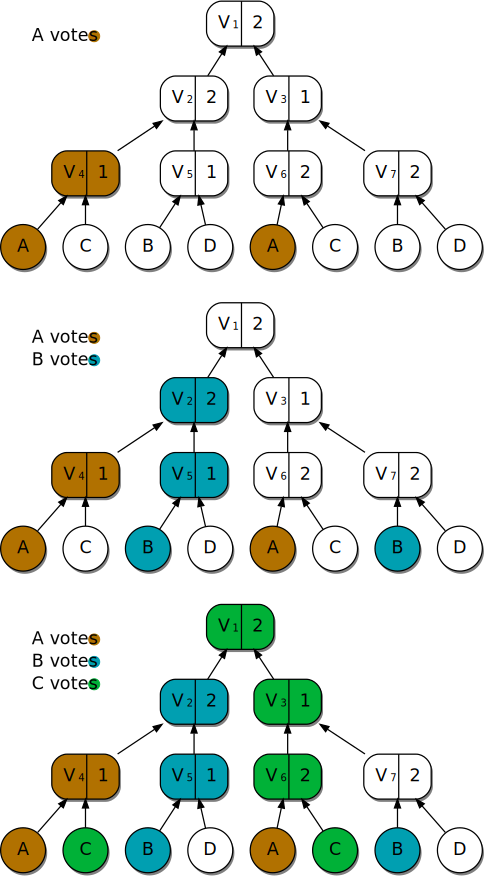
\includegraphics[height=\dimexpr \textheight - 9\smallbaselineskip \relax, keepaspectratio]{Images/Grid4-state.pdf}
    \caption[A vote using the Grid Protocol]{A vote using the Grid Protocol. Each node has one vote. \texttt{A} votes first (maroon). \(V_4\) has a threshold of one, so it votes as well. \(V_2\) and \(V_6\) both have threshold two, so their votes are pending. Then \texttt{B} votes (blue), triggering a vote from \(V_5\). Now both \(V_4\) and \(V_5\) have voted, so \(V_2\)'s threshold of two is reached and it votes, too. At this stage, \(V_1\) and \(V_7\) each require one more vote. Lastly, \texttt{C} votes (green). \(V_4\) has already voted, so nothing happens in this branch. \(V_6\) receives a second vote, so it passes its vote to \(V_3\), immediately triggering it to vote to the root node \(V_1\), where the threshold is now reached, ending the vote.}
    \label{fig:grid4-state}
\end{figure}

Another data type is used in the structured voting code to represent the \emph{state of a vote}. Both are implemented as record types in Erlang, and are called \texttt{vstruct} and \texttt{vstate}, respectively; their internal structure is very similar (see \cref{lst:voting-types} for the full definition). \texttt{vstate} additionally contains information about if and how a physical node has voted (\texttt{true}, \texttt{false} or \texttt{pending}, corresponding to \emph{\yes{} vote received}, \emph{\no{} vote received}, and \emph{not yet voted}, respectively), and a summary of the children's votes for each virtual node (represented as integer fields \texttt{yes\_nodes} and \texttt{no\_nodes}). They are used as follows:

\begin{enumerate}
    \item A \emph{voting structure generator} creates a \texttt{vstruct}.
    \item This voting structure is used to initialise a new voting state \texttt{vstate}.
    \item The voting state is updated by the voting algorithm whenever new votes arrive until the vote succeeds or fails.
\end{enumerate}

The core voting algorithm as illustrated in \cref{fig:grid4-state}, in combination with the \texttt{vstate} data structure described above, lends itself well to a recursive implementation: After looking up the paths in the identifier--path dictionary, the function recurses into the tree along the path and updates the vote at the leaf. After the recursive call, it updates the \texttt{yes\_votes} and \texttt{no\_votes} fields of the virtual nodes along the path. The resulting \texttt{vstate} is then returned.

A vote is finished when it either succeeds or fails. It succeeds when the root node of the tree-shaped voting structure votes \yes; it fails when the root vote \no. The voting algorithm I implemented uses a small optimisation to fail early, that is, to vote \no{} as soon as a quorum for \yes{} cannot be reached. This works as follows: when a child node votes \no, its parent node check whether the threshold is greater than the maximum number of \yes{} votes that can still be cast: \[ \text{threshold} \overset{?}{>} \text{possible \yes{} votes} = \text{number of children} - \text{\no{} votes received}\] If that is the case, then a quorum cannot be formed and the node votes \no.

\section{Voting structure and voting state visualiser}
\label{sc:visualiser}

Once the Erlang representation of voting structures and voting states was fixed, I wrote a visualiser module for them. This allowed me to visually debug my voting algorithm and the voting structure generators.

The visualiser module generates output in the \textsc{dot} graph description language. A \textsc{dot} node is written out for each node in the tree, and edges connect parents and their children. The \texttt{dot} program, which is part of the Graphviz package from \textsc{at\&t} Labs Research, was then used to create \textsc{pdf} or \textsc{svg} files for display.\footnote{Graphviz (short for Graph Visualisation Software): \url{http://graphviz.org}}

Many of the tree diagrams in this dissertation were created using this visualisation tool and then edited and annotated using Inkscape.\footnote{Inkscape is an open source vector graphics editor. \url{http://inkscape.org}}

\section{Voting structure generators}
\label{sc:voting}

In this section, I will describe how the voting structure generators for the three voting protocols I implemented work. These generators output tree-shaped voting structures, which are universal in expressing quorum systems \autocite{structures}. The challenge in building them is to translate the protocol specifications into tree-shaped voting structures.

To simplify this translation, I will now introduce two common patterns that will be used in the description of the Grid Protocol and the Tree Quorum Protocol: \emph{any}- and \emph{all}-nodes.\footnote{Note that the terms any-node and all-node are not used in structured voting literature, but I found them very helpful when designing or reading voting structures.}

\begin{figure}[h]
    \centering
    \begin{subfigure}[t]{0.41\textwidth}
        \centering
        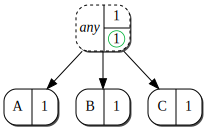
\includegraphics[scale=.75]{Images/Any.pdf}
        \caption{An any-node has a threshold of one, so it votes as soon as \emph{any} of its children do.}
        \label{fig:any}
    \end{subfigure}
    \quad
    \begin{subfigure}[t]{0.41\textwidth}
        \centering
        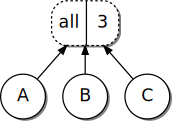
\includegraphics[scale=.75]{Images/All.pdf}
        \caption{An all-node's threshold equals the number of its children, so it requires \emph{all} of them to vote.}
        \label{fig:all}
    \end{subfigure}
    \caption{Common patterns in tree-shaped voting structures.}
    \label{fig:tsvs-patterns}
\end{figure}

Any-nodes have a threshold of one. This means that they pass their vote to their parent as soon as any of their children vote. In logical terms, any-nodes express a logical \emph{or}: In \cref{fig:any}, the root votes if and only if \texttt{A} \emph{or} \texttt{B} \emph{or} \texttt{C} vote. More formally, if for a process \(p\), \(p = \text{true}\) denotes that \(p\) votes \yes,

\[ \text{any-node} = \bigvee_{p\,\in\,\text{Children}} p \]

By contrast, all-nodes have a threshold equal to the number of children they have, so they vote when all their children have voted. In this sense, all-nodes are the tree-shaped voting structure equivalent of the logical \emph{and}: The root in \cref{fig:all} votes if and only if \texttt{A} \emph{and} \texttt{B} \emph{and} \texttt{C} vote. Taking the same mapping between truth assignments and voting as above,

\[ \text{all-node} = \bigwedge_{p\,\in\,\text{Children}} p \]

In the following, \(n\) refers to the total number of processes.

\subsection{Majority Protocol}
\label{ssc:majority}

The Majority Protocol (also know as Majority Consensus Voting\autocite{majority}) requires quorums to contain any \(\left\lceil (n + 1) / 2 \right\rceil\) processes. This makes it an unstructured voting protocol. However, unstructured voting protocols can be regarded as a subclass of structured voting protocols, since they fit into the same framework of voting structure generators.

\begin{figure}[h]
    \centering
    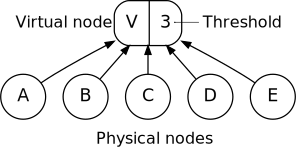
\includegraphics[scale=.75]{Images/Majority5.pdf}
    \caption{Voting structure for the Majority Protocol with five processes.}
    \label{fig:majority5-struct}
\end{figure}

This voting structure has a rigid format, and therefore lends itself to a straightforward implementation: It consists of \(n\) physical nodes, all sharing the same virtual parent node which also acts as the root of the tree-shaped voting structure. Each physical node has one vote, and the threshold of the root node is \(\left\lceil (n + 1) / 2 \right\rceil\), so the vote is decided as soon as this many physical nodes vote \yes.

An example for a Majority Protocol voting structure with five processes and a corresponding threshold of three is given in \cref{fig:majority5-struct}.

\subsection{Grid Protocol}
\label{ssc:grid}

The Grid Protocol was introduced in the Preparation chapter as an example of a structured voting scheme (see \cref{voting-example}). It arranges processes in a logical rectangular grid \autocite{grid}; a quorum consists of one process from each column plus all processes from a complete column.

Assuming for now that our nodes fit into a rectangular \(c \times r\) grid so that \(n = c r\) we can translate the requirements of this specification into a voting structure as follows:

\begin{description}
    \item[\enquote{one process from each column}] This means that for each column, there must be one process which has voted. The literature calls this the \textsc{c}-cover, for \emph{column cover}. In logical terms, it can be expressed as \(\bigwedge_c \bigvee_{p\,\in\,c} p \), where \(c\) ranges over the columns.

        Using the analogy between logic and tree-shaped voting structures introduced at the beginning of this section, we can translate this formula into a voting substructure as follows: for each column \(c\), there is an any-node whose children are the processes in that column (this models \(\bigvee_{p\,\in\,c} p \)). The root of the substructure is an all-node, which has the any-nodes as its children, giving \(\bigwedge_c \bigvee_{p\,\in\,c} p \) altogether. This structure is the \enquote{\textsc{c}-cover subroot} in \cref{fig:grid4-covers}.

    \item[\enquote{all processes from a complete column}] Translating this requirement (called \textsc{cc}-cover for \emph{complete column cover}) into logic, we have \(\bigvee_c \bigwedge_{p\,\in\,c} p \).

        We transform this expression into a tree-shaped voting structure as follows: for each column \(c\), we add an all-node whose children are the processes in that column (giving \(\bigwedge_{p\,\in\,c} p \)). These all-nodes are given an any-node as their parent, modelling \(\bigvee_c \bigwedge_{p\,\in\,c} p \). This node is called \enquote{\textsc{cc}-cover subroot} in \cref{fig:grid4-covers}.
\end{description}

\begin{figure}[h]
    \centering
    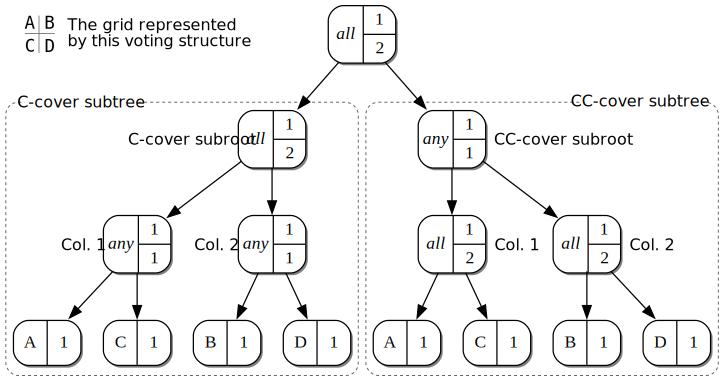
\includegraphics[scale=.75]{Images/Grid4-covers.pdf}
    \caption{Annotated voting structure for the Grid Protocol with four processes.}
    \label{fig:grid4-covers}
\end{figure}

The Grid Protocol specification demands that both requirements must be fulfilled in order to reach a quorum. We thus make the \textsc{cc}-cover root and the \textsc{c}-cover root the children of an all-node as in \cref{fig:grid4-covers}, giving \( \left[ \bigwedge_c \bigvee_{p\,\in\,c} p \right] \wedge \left[ \bigvee_c \bigwedge_{p\,\in\,c} p \right] \), as required. Note how the tree-shaped voting structure resembles the abstract syntax tree of the logical expression.

\minisec{Dealing with incomplete grids}

In the description of the Grid Protocol above, we assumed that the number of processes \(n\) fits nicely into a rectangular grid with \(r\) rows and \(c\) columns. We can of course always enforce this, even when the number of processes is prime, by letting either \(r = 1\) or \(c = 1\). In these extreme cases, however, the Grid Protocol reduces to a voting scheme that requires the consent of \emph{all} nodes for each operation:

\begin{description}
    \item[\(\mathbf{r = 1}\)] makes the \textsc{c}-cover equal to the set of all nodes;
    \item[\(\mathbf{c = 1}\)] makes the \textsc{cc}-cover equal to the set of all nodes.
\end{description}

This is clearly not desirable. Instead, the grid structure imposed on the processes is the smallest almost-square grid that all processes can fit in.\footnote{Almost-square here means that \(c\) and \(r\) differ by at most one, so \(|\,c - r\,| \leq 1\).} Specifically, \( r = \left\lceil \sqrt{n} \right\rceil \) and

\begin{equation}
    c =
    \begin{cases}
        \;\left\lfloor \sqrt{n} \right\rfloor
                 & \text{if } \left\lceil \sqrt{n} \right\rceil
                        \cdot \left\lfloor \sqrt{n} \right\rfloor \geq n \\[0.5em]
        \;\left\lceil \sqrt{n} \right\rceil & \text{otherwise}
    \end{cases}
    \label{eq:grid-dims}
\end{equation}

Note that this implies \(r \geq c\); we are said to be \enquote{favouring rows}. Swapping \(r\) and \(c\) results in grids \enquote{favouring columns}.

The slots in the grid that are not taken up by a process are then considered to be populated by dead placeholder processes. As a little optimisation, we can remove the \textsc{cc}-covers for the columns that contain a placeholder since those columns can never be complete.

\subsection{Tree Quorum Protocol}
\label{ssc:tree}

The Tree Quorum Protocol \autocite{tree} comes in many flavours which allows for different trade-offs between read and write quorum size to be made.\footnote{Remember that \emph{read quorums} are minimal subsets of the cluster that have to vote \yes{} in order for a \emph{read} operation to be performed; \emph{write quorums} are defined analogously.} For my voting structure generator, I picked the variant with the smallest write quorums called \enquote{log write protocol} in which the cardinalities of write quorums are \emph{log}arithmic in the total number of nodes.\footnote{The \enquote{log write protocol} comes with the smallest write quorums and the largest read quorums of all possible Tree Quorum Protocol configurations. The latter should generally to be avoided, but for the purposes of this project, the size of read quorums does not matter since they are disregarded: only write quorums are used for the leader elections.}

In this protocol, the processes are logically arranged in a tree of degree \(d\) (meaning that every parent has \(d\) children). For now, we assume that the tree is complete, that is, it has the maximum number of nodes. A quorum is then defined as any set of nodes forming a path from the root to any leaf of the tree.

\begin{figure}[h]
    \centering
    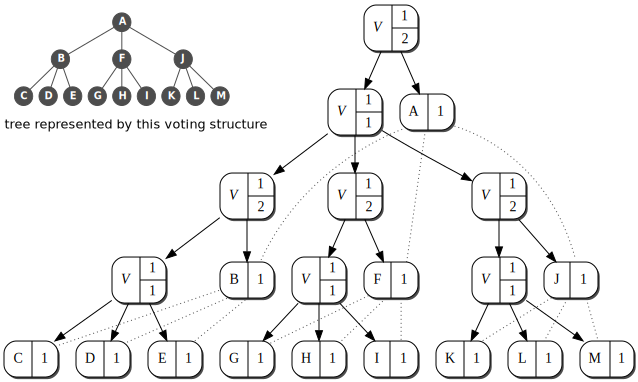
\includegraphics[scale=.75]{Images/Tree3_13.pdf}
    \caption{Voting structure for the Tree Quorum Protocol based on a ternary tree with 13 processes. Processes \texttt{A}, \texttt{F} and \texttt{G} have voted \yes. They lie on a path from the root (\texttt{A}) to a leaf (\texttt{G}), so they form a quorum. \emph{(i) -- (iv)} refer to the description on \cpageref{p:tree-explanation}.}
    \label{fig:grid3_13}
\end{figure}

Take the tree in the top left-hand corner of \cref{fig:grid3_13} as an example. \label{p:tree-explanation}Building the voting structure bottom-up, we start by assembling a substructure representing the subtree with root \texttt{B}. This substructure should only vote if \texttt{B} and one of \texttt{C}, \texttt{D} or \texttt{E} have voted: \( \texttt{B} \wedge \bigvee_{p\,\in\,\text{Children}(\texttt{B})} p \). We can model this easily in terms of any-nodes and all-nodes: \texttt{C}, \texttt{D} and \texttt{E} are given an any-node as their parent -- \emph{(i)} in \cref{fig:grid3_13} --, and this any-node and \texttt{B} are made the children of an all-node \emph{(ii)}.

We proceed in the same way for the subtrees rooted in \texttt{F} and \texttt{J} \emph{(iii)}, and then for the entire tree with \texttt{A} at its root and \texttt{B}, \texttt{F} and \texttt{J} as its children \emph{(iv)}.

Note that this is the only truly recursive tree-shaped voting structure: Majority Protocol voting structures always have a height of two, and any Grid Protocol voting structure is four nodes high. Tree Quorum voting structures, on the other hand, have height \(\left \lceil \log_d{n+1} \right \rceil\) for \(n\) nodes.

\section{Integration with Rafter}
\label{sc:rafter-integration}

Having written and tested the structured voting code, I integrated it into Rafter. This process took place in rougly the following steps:

\begin{enumerate}
    \item Integrating my code with Rafter meant reading and understanding its source code first: 1,500 lines of code\footnote{As measured by \texttt{cloc} (\url{http://cloc.sourceforge.net}).} (see \cref{sc:fp-note} for a discussion of Erlang's code density), spread over 11 modules and undocumented except for a few comments, in a language I was still learning. Using module and function names as a guide, I found the relevant pieces of code that needed changing. Andrew Stone, the developer of Rafter, helped me understand the purpose of a few functions whose task I could not figure out myself.
    \item I renamed my modules and moved them into the appropriate directory to fit into the naming scheme and directory structure of Rafter. Also, the type specifications had to be pasted into the appropriate include file.
    \item In order to use my structured voting code, the node configuration had to be changed from a list of peers (which is all that is needed when only the Majority Protocol is used) to a voting structure (enabling Rafter to use other protocols as well). This required updating every line of code that made use of this field from the configuration record.
    \item All the places in the code which implicitely assumed that the Majority Protocol was being used had to be rewritten. In most cases, this meant making them wrappers around my generalised structured voting code.
\end{enumerate}

\section{Memcached frontend}

\begin{figure}[p]
    \centering
    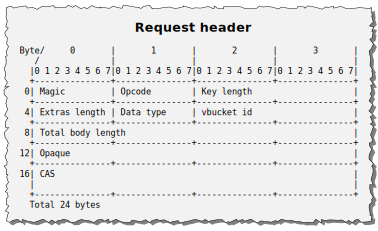
\includegraphics[width=0.7\textwidth, keepaspectratio]{Images/Request_header.pdf}
    \caption[Request header format in Memcached's revamped binary protocol]{Request header format in Memcached's revamped binary protocol.
        \attrib{\url{https://code.google.com/p/memcached/wiki/BinaryProtocolRevamped}}
    }
    \label{fig:request-header}
\end{figure}

\begin{listing}[p]
    \begin{erlangcode}
case Packet of
    <<_Magic:8,    Opcode:8,    KeyLen:16,
      ExtrasLen:8, _DataType:8, _BucketId:16,
      BodyLen:32,
      Opaque:4/binary,     % binary: 4 bytes = 32 bits
      _CAS:64,             % request header ends here
      Body:BodyLen/binary, % request body
      Next/binary>> ->     % start of next request header
        case {Opcode, ExtrasLen, Body} of
            {?NOOP, 0, <<>>} ->
                % handle noop
            {?GET,  0, <<Key:KeyLen/binary>>} ->
                % handle get
            {?SET,  8, <<Flags:4/binary, Expiry:32, Key:KeyLen/binary,
                         Value/binary>>} ->
                % handle set
        end
end
    \end{erlangcode}
    \caption[Request decoding in Erlang]{Memcached request decoder implementation for the binary protocol described in \cref{fig:request-header}. The structure of the \texttt{case Packet} reflects the structure of the packet header. Note how the variable \texttt{BodyLen} captured in the case statement can be used to specify the size of the \texttt{Body} variable within the same case statement. Variables preceded by an underscore are unused.}
    \label{lst:request-header}
\end{listing}

Memcached is a high-performance key-value cache designed to sit between an application and a database. If the application issues a query that has been seen before by Memcached, the result is served from the cache; otherwise, the query is executed on the database and the result stored in Memcached. Originally developed for LiveJournal, Memcached is now used by many high-traffic websites including Youtube, Twitter, Reddit, Facebook and Wikipedia.

My implementation of a Memcached frontend for Rafter amounts to a slight abuse of Memcached for my own intentions. First and foremost, Memcached caches are designed to be very fast, at the expense even of durability: clients cannot, in general, expect the cache to keep a value in memory indefinitely -- dropping a key-value pair to make place for a new one is perfectly acceptable for a cache like Memcached. Rafter, in contrast, is designed to be durable: every write operation is flushed to disk at once. Therefore, building a Memcached protocol frontend on top of it results in an implementation that is orders of magnitude slower than original Memcached and has different eviction semantics.

I added a Memcached frontend to Rafter for two reasons: to showcase a useful application that could be built on top of it, and to be able to use Memcached's benchmarking tool, \texttt{memaslap}.\footnote{\texttt{memaslap} is part of libMemcached (\url{http://libmemcached.org/libMemcached.html}), an open source library and toolset for Memcached.}

Newer versions of Memcached support a binary protocol,\footnote{Memcached's new binary protocol is described in this document: \url{https://code.google.com/p/memcached/wiki/BinaryProtocolRevamped}.} which I found less ambiguous than the standard text-based protocol. Decoding and encoding binary protocols being a particular strength of Erlang, the decision over which protocol to implement was easy. \Cref{lst:request-header} illustrates how the decoding of a Memcached request is implemented.

Next, I picked the commands and features I wanted the frontend to support. Since my store is meant to be a proof-of-concept, I decided to stick to the minimal set of commands required for a key-value store: \texttt{get}, \texttt{set}, and \texttt{noop}, with the obvious meaning: \texttt{get} is a read request, \texttt{set} starts a write operation and \texttt{noop} does nothing. For simplicity, I also decided not to support the data version check feature (the \textsc{cas} header field in \cref{fig:request-header}).

\minisec{Implementing Memcached}

The actual implementation of the Memcached frontend consists of three parts: A supervisor, a protocol decoder/encoder, and a backend.

\begin{description}
    \item[The supervisor] starts and watches over instances of the decoder/encoder. \emph{Supervisors} are a \emph{behaviour} defined in the \textsc{otp}, Erlang's set of core libraries. Crucially, they are notified when a process started by them fails. By default, the Memcached supervisor starts 20 instances of the decoder/encoder, which allows up to 20 clients to connect to the server simultaneously.\footnote{My measurements show that increasing the number of decoders above 20 does not significantly improve the throughput.} Whenever one of them crashes, a new decoder/encoder is brought up.
    \item[The protocol decoder and encoder] makes up the actual \enquote{frontend}: this is the component a Memcached client talks to directly via \textsc{tcp}.
    \item[The backend] finally executes the commands decoded by the frontend by reading from and writing to a local database. In Raft terminology, this module constitutes the \emph{state machine}. It uses Erlang's built-in \texttt{ets} (Erlang Term Storage) module for storing the data.
\end{description}

\section{Failure simulation}

In order to evaluate and compare the different voting structures, I added failure simulation to Rafter's state machine. Apart from being in leader, follower or candidate state, nodes can now also be in the \textit{failed} state. Failed nodes do not process any incoming messages, nor do they send any messages to other nodes.

According to Jeff Dean of Google, two of the most common failure modes in a modern data centre are individual machine failures (called \emph{repeated failures} in the following) and rack failures (correlated failures) \autocite[sl. 10]{distr}. During a preliminary theoretical analysis, I could find no evidence that structured voting schemes would be able to deal with rack failures better than unstructured protocols. Hence only repeated/individual failures were considered.

% The failure simulation, like all the benchmarking code I wrote for this project, assumes that the leader is fixed and stays up. This leader can then instruct its followers to fail -- either once or repeatedly. It is, in turn, controlled by the \emph{benchmark runner}, which is the Amazon \ECC instance that runs the benchmarking scripts. For the \textbf{fail once} \label{fail-once} failure mode, the process is as follows:

% \begin{enumerate}
    % \item The benchmark runner sends a message to the leader with parameters \(\lambda\) and \(T\).
    % \item After waiting for a time \(t \sim \text{Exp}(\lambda)\), the leader sends a message to a random follower to go into failed state for time \(T\).
    % \item The leader repeats step (2.) until it receives a \enquote{stop} message.
% \end{enumerate}

Here is how I implemented \label{repeated-failures} \emph{repeated failures}: the idea is that a parameter \(\texttt{Up} \in \oiv{0,1}\) specifies the uptime ratio of each node. After running for a time \(t \sim \text{Exp}(\lambda)\), nodes fail for time \(t \cdot \frac{1 - \texttt{Up}}{\texttt{Up}}\). This results in followers being \enquote{up}, that is, actively participating in the cluster, for approximately \(\texttt{Up} \cdot 100\%\) of the time:
\[ \frac{\text{uptime}}{\text{total time}}
 = \frac{\text{uptime}}{\text{uptime} + \text{duration of failure}}
 = \frac{t}{t + t \cdot \frac{1-\texttt{Up}}{\texttt{Up}}}
 = \frac{\texttt{Up}}{\texttt{Up} + 1 - \texttt{Up}} = \texttt{Up} \]

Since \(t\) is an inter-event time, generating it using an exponential distribution is an obvious choice. Erlang's core libraries provide a function for generating uniformly distributed floating point numbers \(U \sim \text{U}(0,1)\). Using the formula introduced in the Part \textsc{ii} Computer Systems Modelling course, \(t\) is calculated from \(U\) and the parameter \(\lambda\) as \(t \coloneqq -\frac{1}{\lambda}\log{U}\).

The actual failure simulation then proceeds as follows:
\begin{enumerate}
    \item The benchmark runner sends a message to the leader with parameters \(\lambda\) and \texttt{Up}.
    \item Immediately, the leader sends a message to some or all of its followers to start failing.
    \item On receiving this message, each follower waits for time \(t \sim \text{Exp}(\lambda)\) before transitioning to failed state.
    \item After waiting for time \(t \cdot \frac{1 - \texttt{Up}}{\texttt{Up}}\), the follower goes back to \textit{follower} state.
    \item Followers repeat steps (3.) and (4.) until the leader sends out a \enquote{stop} message.
\end{enumerate}

\section{Logging}

In order to collect benchmarking data, I created a simple logging module. This module implements the \emph{gen\_server} behaviour defined in the \textsc{otp}. It runs in a separate process under its own supervisor. The logger receives messages in a certain format from other components of the system, and writes the values out in a comma-separated values (\textsc{csv}) file. The fields recorded in the \textsc{csv} file are:

\begin{description}
    \item[Experiment] the voting scheme used and its parameters, if any;
    \item[Cluster] the number of nodes in the cluster;
    \item[Operation] \texttt{Read} or \texttt{Write};
    \item[Time to consensus (\textsc{ttc})] the time taken between receiving the request and returning its result to the client in microseconds.
\end{description}

\begin{table}[h]
    \centering
    \begin{tabular}{l c c c}
        \toprule
        \textit{Experiment} & \textit{Cluster} & \textit{Operation} & \textit{\textsc{ttc} (\si{\micro\second})} \\
        \midrule
        \multicolumn{4}{c}{\(\vdots\)} \\
        Majority & 3 & Write & 2920 \\
        Majority & 3 & Read & 2166 \\
        \multicolumn{4}{c}{\(\vdots\)} \\
        Grid & 11 & Write & 9801 \\
        Grid & 11 & Read & 7269 \\
        \multicolumn{4}{c}{\(\vdots\)} \\
        \bottomrule
    \end{tabular}
    \caption[Example TTC log snippet]{Example \textsc{ttc} log snippet}
    \label{tab:csv}
\end{table}

Rafter puts information related to a specific request in a record of type \texttt{client\_req}. For logging purposes, I added a field \texttt{started} to it, which is initialised to the current system time whenever a new client request record is created. I then amended the function sending the client response to also send a message to the logger containing the time difference between the current system time and the time when the request was started.

I conducted a short series of tests to see if turning on logging decreased the performance of Rafter. No statistically significant effect on the throughput could be found. There are two main reasons for this: firstly, as mentioned above, the logger runs in its own process and receives messages from other components of the system. This means that when a process wants to add an entry to the log, it sends a message to the logger. The program flow is not interrupted: the message is simply queued in the logger's message inbox and the process that sent the message continues execution. The logger acts upon the message at some later point when the Erlang scheduler decides to switch to its message handling procedure. Hence the logger automatically benefits from Erlang's scheduling and parallelism features, decreasing the time penalty.

Secondly, the \textsc{cvs} files are written to a folder in \texttt{/tmp}, which is mounted as a \texttt{tempfs} file system. Under normal operating conditions, this complete file system lives in main memory and is never written to disk. This makes write operations very cheap, again keeping the time penalty for logging at a minimum.

\section{Reporting issues and bugs}

During the development of this project, I noticed several issues with the software I was using (see \cref{tab:issues} for a summary). In some cases, this was due to a misunderstanding on my part -- for example, I was having trouble setting up and using QuickCheck, so I contacted Thomas Arts of Quiviq who helped me sort things out. In some cases, I found mistakes in the documentation: when this happened, I forked the project, corrected the mistake, and created a pull request.\footnote{This is the development model used by most projects hosted on GitHub. \emph{Forking} copies the project to one's personal space. The contributor creates a new branch, attempts to fix the bug, and opens a \emph{pull request} for that branch. A pull request can then be reviewed, discussed and amended until it is either rejected or accepted and merged into the original project's \texttt{master} branch.} This caused me to create pull requests for Rafter, StatsBase.jl, a statistics package for the scientific programming language Julia that I used to analyse the benchmarking data, and awsfabrictasks.

\ctable[
    caption = Issues found with third-party software during the development of the project,
    label = tab:issues,
    width = \textwidth,
    pos = ht
]{Xp{.72\textwidth}}{
    \tnote[a]{Issue report: \url{https://github.com/andrewjstone/rafter/issues/22},

        Pull request: \url{https://github.com/andrewjstone/rafter/pull/23}}
    \tnote[b]{Pull request: \url{https://github.com/andrewjstone/rafter/pull/17}}
    \tnote[c]{Issue report: \url{https://github.com/espenak/awsfabrictasks/issues/15}}
    \tnote[d]{Issue report: \url{https://github.com/espenak/awsfabrictasks/issues/17}}
    \tnote[e]{Pull request: \url{https://github.com/espenak/awsfabrictasks/pull/16}}
    \tnote[f]{Pull request: \url{https://github.com/JuliaStats/StatsBase.jl/pull/48}}
}{  \FL
    \textit{Project} & \textit{Issue} \ML
    \vspace*{-3pt}\multirowbt{2}{*}{Rafter}
        & \textsc{cpu} usage and operation execution time increase with the number of operations performed\tmark[a] \NN
    \cmidrule(l){2-2}
        & More consistent variable naming in \textsc{readme}\tmark[c] \ML
    \multirowbt{3}{*}{Awsfabrictasks}
        & \texttt{\@ec2instance} decorator executed too early\tmark[c] \NN
    \cmidrule(l){2-2}
        & \texttt{\@ec2instance} login problem\tmark[d] \NN
    \cmidrule(l){2-2}
        & Documentation correction\tmark[e] \ML
    StatsBase.jl & Corrections in \textsc{readme}\tmark[f] \LL
}

Apart from these issues, I found two actual bugs in the software I was using. The first one concerned the performance of Rafter: I noticed that both read and write operations took more and more time the longer Rafter had been running for. I wrote a small test script, took some measurements and reported the problem to Andrew Stone, the original author of Rafter, who responded quickly and managed to fix the issue within a few days.

The second larger issue I found was a problem with a very common use case that was not well addressed in awsfabrictasks's \textsc{api}. I reported this to the software's author, Espen Angell Kristiansen; eventually, this discussion turned into a proper bug report.

\section{Summary}

In this chapter, I described the implementation of the structured voting extension for Rafter, and the set-up required for benchmarking. The chapter started with a description of the data types used to represent voting structures and voting state. I briefly talked about the visualiser, which was used to visually debug the voting algorithms and the voting structure generators.

The voting structures for the Majority Protocol, the Grid Protocol and the Tree Quorum Protocol were derived and explained. I described the process of integrating my structured voting code into Rafter before detailing the two extensions to Rafter I implemented to make benchmarking possible: the Memcached frontend and failure simulation. Finally, I mentioned the bug reports and pull requests I created for various pieces of software I used in this project.



\chapter{Evaluation}
\label{ch:evaluation}

% \begin{itemize}
    % \item Signs of success, evidence of thorough and systematic testing
    % \item Sample output, graphs, diagrams
    % \item Original goals achieved? Proof? Did stuff work?
% \end{itemize}

% \begin{itemize}
    % \item Failure modes presentation: most frequent failure modes are individual, then rack failures
% \end{itemize}

\section{Overall results}
\label{sc:overall-results}

All the success criteria listed in my project proposal have been met, and in some areas, I have gone beyond what the criteria demanded (see XXX.)

\begin{enumerate}
    \item \emph{Design of the data structure to represent voting structures, and implementation and testing of the algorithm to interpret it.}

        These goals were tackled first, since all other components depend on the voting structure and state type specification and the core voting algorithm being implemented successfully (see \cref{fig:dependencies}.) For the relevant background, see \cref{ssc:structured-voting-schemes}; the implementation is described in \cref{sc:voting-algo}.
    \item \emph{Implementation and testing of voting structure generators for at least Majority Voting and the Grid Protocol.}

        Voting structure generators for Majority Voting and the Grid Protocol were implemented successfully. Additionally, I wrote a voting structure generator for the Tree Quorum Protocol. They were tested for internal consistency using randomised unit tests, and for correctness by visual inspection using the voting structure visualiser discussed in \cref{sc:visualiser}.

        The theory behind voting schemes is introduced in \cref{ssc:structured-voting-schemes}, the implementation of the three voting structure generators is described in \cref{sc:voting}.
    \item \emph{Incorporating the above algorithms and data structures into Rafter so they can be used to find quorums.}

        Integration with Rafter has been accomplished, and I have demonstrated that Rafter can run using my voting code to elect the leader. \Cref{ssc:raft-consensus-algorithm} provides the background on Raft, and \cref{sc:rafter-integration} describes the integration process.
    \item \emph{Setting up the project so it can be run as a distributed key-value store in the Amazon Elastic Compute Cloud infrastructure.}

        I took an Arch Linux image specially made to run on Amazon \ECC{} instances, built and installed all necessary tools required for benchmarking, and deployed it on a cluster.
    \item \emph{Running the benchmarks, and collecting and evaluating the results. The evaluation must include a comparison and discussion of the benchmarks collected for the different voting schemes.}

        See \cref{ssc:results}.
\end{enumerate}

\section{Testing}

In the early stages of the development of each component, testing was primarily manual. Once the code had reached a stage where testing by hand did not uncover any more bugs, I wrote a QuickCheck test for that component.

The QuickCheck tests, in their simplest form, consist of \emph{generators} (not to be confused with voting structure generators) and a set of functions specifying the \emph{properties} of the generated objects (examples for both are given in \cref{sc:testing-examples}.) QuickCheck then randomly instantiates test cases using the generators, and checks if they behave as expected.

Voting structure generators, in particular, were tested using two complementary methods: visually, I checked them for correctness using the voting structure visualiser (see \cref{sc:visualiser}); a QuickCheck property tested for internal integrity.

\begin{table}[h]
    \centering
    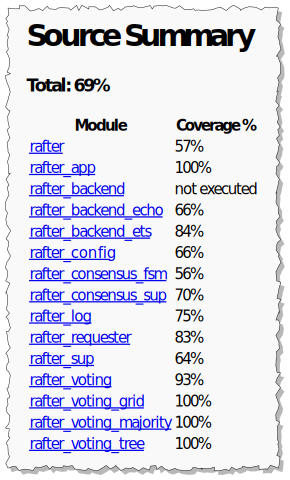
\includegraphics[height=0.45\textheight, keepaspectratio]{Images/Coverage_summary.pdf}
    \caption[Unit test coverage]{Unit test coverage of the structured voting code. Note in particular the high coverage of the last four modules, which were written as part of this project.}
    \label{tab:coverage}
\end{table}

\Cref{tab:coverage} shows a screenshot of the test coverage report for the project generated by the EUnit library. I modified four out the five original test modules and added another four to cover my structured voting code. Of the modules shown, I edited \texttt{rafter\_config}, \texttt{rafter\_consensus\_fsm} and \texttt{rafter\_consensus\_sup} and wrote the bottom four modules (all starting with \texttt{rafter\_voting}) from scratch.

\section{Benchmarking}

In order to compare the performance of my voting algorithms with those used in the original Rafter code, and to see how different voting schemes scale with the number of nodes, I designed, scripted and ran a series of benchmarks in the Amazon Elastic Compute Cloud. Overall, it took me over a month to set everything up in a way such that useful data could be acquired.

\subsection{Helper scripts}
\label{ssc:benchmarking-scripts}

\begin{figure}[p]
    \centering
    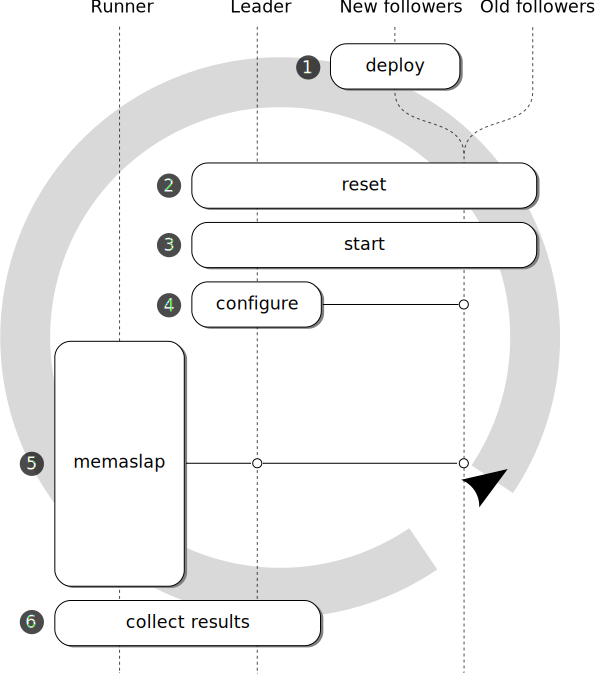
\includegraphics[scale=.75]{Images/Benchmarking.pdf}
    \caption[Benchmarking flowgraph]{High-level overview of the \emph{benchmark} task:
    \begin{inparaenum}[(1)]
        \item The latest version of the source code is pulled from the central repository and compiled on the new followers.
        \item On all followers and the leader, the Erlang process is killed and the file system cache is purged.
        \item Rafter is started on each node in the cluster.
        \item The leader is configured. This step triggers a leader election.
        \item Memaslap is executed on the runner, targeting the leader.
        \item The script downloads log files from the runner and the leader.
    \end{inparaenum}
    }
    \label{fig:benchmarking}
\end{figure}

The benchmarks are automated using Fabric and the awsfabrictasks plugin (see \cref{ssc:ec2-benchmarking} for a brief description of the two software packages). A task called \textit{benchmark} executes a sweep of the parameter space, starting nodes as appropriate and collecting the logged results. It makes use of a few helper functions:

\begin{description}
    \item[deploy] Executes a series of Git commands on the remote instance to bring the project repository up to date and to a specific branch. It then runs \texttt{make} to build the project.
    \item[start\_erlang\_node] Takes a name as its parameter and starts an Erlang node with that name on the instance.
    \item[stop\_erlang\_node] Kills the Erlang interpreter process on this instance.
    \item[configure] Creates a configuration script and executes it. The script evaluates an Erlang program that is created on the fly. It uses Erlang's remote procedure call module, to issue a call to the leader to update its configuration, which consists of the list of followers and the voting scheme to use. The script then sends a message to the leader to relay a \enquote{restart} message to its followers so they all recover from a possible failed state. Finally, a new failure mode is sent to the leader.
    \item[memaslap] Runs \texttt{memaslap}, the Memcached load tester, locally, targeting the Memaslap frontend running on the leader node. The output of the program is diverted into a log file.
    \item[collect\_results] Uses \texttt{rsync} to download the Memcached and time to consensus log files to the machine running the benchmarks.
\end{description}

The \textit{benchmark} task uses these helper functions as follows: For each combination of cluster size, protocol and failure mode that is to be tested, the procedure starts by deploying the latest version of the project source code to all instances as required and compiling it (using the \texttt{deploy} task). It then starts up an Erlang node with a fresh name on each of them. These nodes start in follower state and with an empty initial configuration.

Next, the leader is reconfigured using the \texttt{configure} task. Then \texttt{memaslap} is run, and its results as well as the time to consensus measurements are downloaded by the \texttt{collect\_results} task. See \cref{fig:benchmarking} for a visualisation of the complete benchmarking procedure.

\subsection[Amazon EC2 set-up]{Amazon \ECC set-up}

New instances in the Amazon Elastic Compute Cloud are created from virtual appliances called \enquote{Amazon Machine Images} (\textsc{ami}s). Amazon's own default \textsc{ami} does not have the latest version of the Erlang platform in its package sources, so I based my custom \textsc{ami} on an Arch Linux image instead.\footnote{Project \enquote{Arch Linux on \ECC}: \url{https://www.uplinklabs.net/projects/arch-linux-on-ec2/}} I created an instance of the Arch \textsc{ami}, installed Erlang and a few standard tools and built libMemcached from source, as all distributions I checked had building \texttt{memaslap} disabled by default.

Users of the Amazon Elastic Compute Cloud currently have the choice between many different instance types. Preliminary experiments using a cluster of (free) \enquote{micro} instances were useful for learning how to use the Amazon \ECC administration tools, but their performance turned out to be too low, and \textsc{ssh} connections were flaky. At the recommendation of my project supervisors, I switched to \enquote{m1.xlarge} general-purpose instances for running the benchmarks (see \cref{tab:instance-types} for a comparison.)

The m1.xlarge instances provided enough compute power and much more network bandwidth than the micro instances. Connections to them were reliable once established. Occasionally, \textsc{dns} lookup errors occurred. This was a major annoyance, but the problems were always fixed within a few hours.

\begin{table}[h]
    \centering
    \begin{tabularx}{\textwidth}{X c c S c c}
        \toprule
        \textit{Name} & \textit{\textsc{ecu}s} &
        \textit{v\textsc{cpu}s} & \textit{Memory (\textsc{g}i\textsc{b})} &
        \textit{Storage (\textsc{gb})} & \textit{Network performance} \\
        \midrule
        t1.micro & up to 2 & 1 & 0.613 & \textsc{ebs} only & very low \\
        m1.xlarge & 8 & 4 & 15 & 4 \(\times\) 420 & high \\
        \bottomrule
    \end{tabularx}
    \caption[Comparison of Amazon \ECC instance types]{Comparison of the two Amazon \ECC instance types used. \textsc{ecu} stands for \enquote{Elastic Compute Unit}, roughly equivalent to one 1.0 \textsc{gh}z 2007 Opteron; a v\textsc{cpu} is a virtual \textsc{cpu}; \textsc{ebs} means \enquote{Amazon Elastic Block Storage}.}
    \label{tab:instance-types}
\end{table}

\subsection{Choice of parameters}

Due to time constraints, benchmarking every combination of parameters was impossible. I benchmarked all voting structures. The Grid Protocol was tested with the \enquote{favouring rows} option; benchmarks were also run on binary and tertiary trees created by the Tree Quorum Protocol.

As for cluster sizes, I tried to find configurations for which at least one protocol was optimal in some way. My Amazon \ECC account allowed me to run experiments with up to 19 nodes (plus one separate \enquote{runner} instance).

\begin{description}
    \item[Majority Protocol] Any uneven number of nodes is optimal.
    \item[Grid Protocol] Clusters of size 4, 9 and 16 are square; 6 and 12 form full almost-square rectangles. However, grids of size 4 and 6 require more nodes than the Majority Protocol for a quorum, which makes them less interesting for this analysis.
    \item[Tree Quorum Protocol] Trees of degree \(d\) and height \(h\) with \(n = \sum^h_{i=0} d^i\) nodes are full. Considering cluster sizes less than 20, binary trees of size 3, 7 and 15 are full, and so are ternary trees with 4 or 13 nodes.
\end{description}

Taking the union of the \enquote{interesting} optimal cases, we get 3, 4, 5, 7, 9, 11, 12, 13, 15, and~17 as the cluster sizes to benchmark.

\subsection{Empirical results: no failures}
\label{ssc:results}

This section discusses the results gathered from running the benchmarks with failure simulation turned off.

The purpose of the benchmarks was twofold: to find the overhead caused by adding additional complexity in the form of the structured voting layer, and to compare the performance of different structured voting schemes.

\minisec{Comparison with the original Rafter implementation}

\Cref{fig:plain-maj-ttc} shows time to consensus (\textsc{ttc}, y-axis) as a function of the cluster size (x-axis). The two curves have the same shape: this is to be expected, since the quorum finding mechanism works in precisely the same way. The time to consensus for the original Rafter implementation without structured voting schemes (the \enquote{plain} curve in the graph) is consistently smaller, and the difference between the two curves increases with the number of nodes in the cluster. In other words, for clusters with less than 20 nodes at least, computing quorums under the Majority Protocol takes roughly \SI{300}{\micro\second} longer per node than with the original Rafter implementation.

This was to be expected: the voting scheme which is implemented by original Rafter is the same as the Majority Protocol, but the implementation is very different. In the original Rafter code, checking if a quorum has been found amounts to checking whether or not the number of \yes{} votes received is greater than half the number of servers. With the Majority Protocol, on the other hand, a new voting state is created whenever a new vote takes place, and a tree-walking algorithm updates it whenever a new vote comes in. It should come as no surprise that this takes longer.

A more interesting aspect is the seemingly linear relationship between the size of the cluster and the difference in time to consensus between the Majority Protocol and original Rafter. This can be explained as follows: whenever a new vote comes in, the root node \enquote{accumulates} all votes, that is, it updates the number of \yes{} and \no{} votes it has seen by looking at its children. But the number of children of the root node in the Majority Protocol voting structure is precisely the size of the cluster, which means that for every incoming node, updating the voting state takes \(O(n)\) time.

\minisec{Comparison between different structured voting schemes}

\begin{figure}[p]
    \begin{subfigure}{1\textwidth}
        \centering
        \includegraphics[width=0.75\textwidth, keepaspectratio]{Images/ttc_plain-maj.pdf}
        \caption{Time to consensus results for original Rafter and the Majority Protocol.}
        \label{fig:plain-maj-ttc}
    \end{subfigure}

    \begin{subfigure}{1\textwidth}
        \centering
        \includegraphics[width=0.75\textwidth, keepaspectratio]{Images/ttc_maj-tree-grid.pdf}
        \caption{\textsc{ttc} measurements for different structured voting schemes}
        \label{fig:maj-tree-grid-ttc}
    \end{subfigure}
    \caption{Time to consensus measurements for the original Rafter implementation (\enquote{plain}), the Majority Protocol (\enquote{majority}), the Tree Quorum protocol (\enquote{tree2} and \enquote{tree3} with branching factors \(d = 2\) and \(d = 3\), respectively), and the Grid Protocol (\enquote{grid}). The lines connect the median measurements and the error bars indicate the 25th and the 75th percentile.}
    \label{fig:ttc}
\end{figure}

The time to consensus versus cluster size graph for all four structured voting schemes implemented in this project in \cref{fig:maj-tree-grid-ttc} has some interesting features.

Consider the graph of the Grid Protocol time to consensus (the \enquote{grid} dataset in \cref{fig:maj-tree-grid-ttc}). The \textsc{ttc} measurements increase by about \SI{3.5}{\milli\second} between 12 and 13 nodes but then stay within about \SI{1}{\milli\second} until the cluster size reaches 16; then there is a jump by \SI{7.5}{\milli\second} as the cluster size hits 17. Why the plateau between 13 and 16? By \cref{eq:grid-dims}, cluster sizes 13, 14, 15, and 16 all generate quadratic 4\,\(\times\)\,4 grids. Clusters with 12 nodes fit into a 4\,\(\times\)\,3 grid, and those with 17 nodes require a 5\,\(\times\)\,4 grid. Thus, it seems that the \textsc{ttc} times change mainly when the grid shape changes.

This behaviour can be explained by looking at the number of nodes required to vote \yes, which depends on the shape of the grid: for a \(r \times c\) grid it is \(r + c - 1\).\footnote{A Grid Protocol quorum needs votes from each column  (\(c\) votes) and one entire column (\(r\) votes). Those two sets intersect in one process, and so the number of processes in a Grid Protocol quorum is \(r + c - 1\).} For cluster sizes 13, 14, 15 and 16, the grid has the same 4\,\(\times\)\,4 shape, so in each case, seven votes are required.

% It is important to note that seven \yes{} votes from arbitrary processes do \emph{not} suffice; rather, \ldots

The Tree Quorum Protocol graphs show a similar behaviour. A cluster of 15 nodes exactly fills a binary tree of height 3. Add one more node, and a non-full binary tree of height 4 is required to hold all nodes. Analogously, 13 nodes fit exactly into a ternary tree of height 2; more nodes require at least height 3. This helps explain the rapid increase in time to consensus between 15 and 16 nodes in the binary (\enquote{tree2}) case and the similar effect between 13 and 15 nodes in the ternary (\enquote{tree3}) case.

\begin{figure}[t]
    \centering
    \includegraphics[width=0.75\textwidth, keepaspectratio]{Images/ttc_grid.pdf}
    \caption{Time to consensus plots for the Grid Protocol. The numbers indicate uptimes in percent: \texttt{grid-80} is the dataset captured with uptime 80\%, and analogously for \texttt{grid-60} and \texttt{grid-40}.}
    \label{fig:ttc-grid}
\end{figure}

\minisec{The dent in the cumulative histogram}

\begin{figure}[p]
    \centering
    \includegraphics[width=0.75\textwidth, keepaspectratio]{Images/ttc_7_plain-maj-tree-grid.pdf}
    \caption{Cumulative histogram of time to consensus measurements for a cluster with seven nodes, under original Rafter, the Majority Protocol, the Tree Quorum Protocol and the Grid Protocol (legend as for \cref{fig:ttc}).}
    \label{fig:plain-maj-tree-grid-ttc}
\end{figure}

All cumulative histograms (\cref{fig:plain-maj-tree-grid-ttc} show the one for a cluster of size 7) of the time to consensus measurements I took exhibit one or more \enquote{dents} between the 75th and the 100th percentile. These show up as large upper error bars in \cref{fig:ttc} as well. Where do they come from?

Preliminary experiments showed that the time to consensus increases by orders of magnitude when the load on the system is high. The system load is primarily a function of the frequency at which the client -- \texttt{memaslap} for the purposes of the benchmarks -- sends requests. By carefully reducing this throughput by varying the \texttt{--tps=X} command line parameter, I made sure to operate the system in a regime just below overloading for most of the requests. This is the part of the curves below the dents, roughly the region below the 75th percentile.

\minisec{Throughput}

Throughput is highly correlated with time to consensus: The lower the \textsc{ttc}, the higher the throughput. But it depends on a number of other factors as well, most importantly the amount of parallelism in the system: if the number of operations that can be executed simultaneously is doubled, then (ceteris paribus) the throughput doubles while \textsc{ttc} stays constant.

I used the output of Memaslap (which \cref{fig:throughput} is compiled from) to confirm that my time to consensus values were reasonable. It is important to note that while \cref{fig:ttc,fig:plain-maj-tree-grid-ttc} show time to consensus for write operations only, \cref{fig:throughput} indicates the throughput averaged over both read and write operations. The reason behind this is that in Rafter, the leader has the canonical log, and can therefore serve any read request directly. There is no quorum-building involved in a read operation, and so the response time is independent of the voting structure or the cluster size. Unfortunately, Memaslap only outputs the overall average throughput, so I had to make do with this one value.

\begin{figure}[p]
    \centering
    \includegraphics[width=0.75\textwidth, keepaspectratio]{Images/throughput.pdf}
    \caption{Throughput for original Rafter and different structured voting schemes (legend as for \cref{fig:ttc}).}
    \label{fig:throughput}
\end{figure}

\subsection{Empirical results: repeated failures}
\label{ssc:repeated-failures}

The repeated failures simulation is described on \cpageref{repeated-failures}. Time to consensus graphs for 80\%, 60\% and 40\% uptime can be found in \cref{sc:ttc-graphs}.

The graphs show that as long as the uptime is above 40\%, time to consensus values do not change significantly. \Cref{fig:ttc-grid} shows an example graph for the Grid Protocol where the lines almost coincide and no general trend can be extracted. The same plot for other structured voting schemes looks similar.

\section{Summary}

This chapter started by showing that all the requirements of the project proposal have been fulfilled. I described my testing set-up using QuickCheck and demonstrated good software engineering practice through very high test coverage.

The remainder of the chapter was devoted to a discussion of the benchmarking measurements. Two main results have been found. Firstly, the implementation of structured voting schemes is computationally more expensive than hard-coding majority voting and therefore slower, as demonstrated by \cref{fig:plain-maj-ttc}. This was to be expected.

Secondly, I have shown that structured voting schemes are nevertheless worth considering in a practical setting. \Cref{fig:maj-tree-grid-ttc-circled} shows that given the right cluster size, structured voting schemes can be faster than unstructured voting schemes in finding quorums, as evidenced by the circled region of the graph. Here, the (ternary) Tree Quorum Protocol, a structured voting scheme, beats the Majority Protocol, the default unstructured voting scheme, in the time to consensus measurements.

\begin{figure}{1\textwidth}
    \centering
    \includegraphics[width=1\textwidth, keepaspectratio]{Images/ttc_maj-tree-grid-circled.pdf}
    \caption{Time to consensus measurements for different voting schemes. This graph shows the main evidence that structured voting schemes can have practical advantages. Within the circled area, the (ternary) Tree Quorum Protocol found quorums significantly faster than the Majority Protocol. This graph is an annotated version of \cref{fig:maj-tree-grid-ttc}.}
    \label{fig:maj-tree-grid-ttc-circled}
\end{figure}



\chapter{Conclusions}
\label{ch:conclusions}

% \begin{itemize}
    % \item Refer to Introduction
    % \item Lessons learnt
% \end{itemize}

This dissertation has described how I designed, implemented, tested and benchmarked a structured voting extension to Rafter, an existing implementation of the new Raft consensus algorithm. All goals outlined in the original proposal have been met, and a few optional extensions have been added.

\minisec{Results}

The result of the project is twofold: firstly, the implementation of the extension itself. I have successfully built upon an existing piece of software, Rafter, that is still in an early phase of development, largely undocumented and written in a language I was entirely unfamiliar with when I started this project. The extension works and is stable. Adding more structured voting schemes is easy.

Secondly, I have shown that structured voting schemes have practical value. The main evidence for this can be found in \cref{fig:maj-tree-grid-ttc-circled}, which shows that under certain conditions, structured voting schemes can be more efficient than unstructured ones. Optimising the voting structure data types and algorithms would decrease the penalty for using structured voting schemes, and therefore result in structured voting schemes being more efficient than unstructured ones under a larger range of configurations, especially as the size of the cluster grows big.

\minisec{Takeaway}

Doing this project and writing the dissertation has been very educational. I have learnt to administer cloud servers, analysed big datasets with a variety of different tools, and fought battles with \LaTeX{} to get just the layout I wanted. Last but not least, I have learnt to appreciate just how much time and care it takes to benchmark a distributed system.

\minisec{Conclusion}

I hope that this dissertation is readable, and that I have given each part of the project appropriate space for explanation and discussion. Structured voting schemes are not a new idea, but maybe after decades of being confined to academic papers, they will finally be picked up by implementers of distributed systems -- the potential for efficiency gains are real, as this dissertation has shown.

%TC:ignore

\printbibliography

% \backmatter

\appendix



\chapter{Additional resources}

\section{Raft safety guarantees}
\label{sc:rafter-safety}

Figure 3 of the Raft paper lists the following safety properties which the algorithm guarantees to be true at all times:\autocite{raft}

\begin{description}
    \item[Election Safety:] at most one leader can be elected in a given term.\footnote{Raft divides time into \emph{terms} of arbitrary length. Each begins with an election, in which one or more candidates attempt to become leader.}
    \item[Leader Append-Only:] a leader never overwrites or deletes entries in its log; it only appends new entries.
    \item[Log Matching:] if two logs contain an entry with the same index and term, then the logs are identical in all entries up through the given index.
    \item[Leader Completeness:] if a log entry is committed in a given term, then that entry will be present in the logs of the leaders for all higher-numbered terms.
    \item[State Machine Safety:] if a server has applied a log entry at a given index to its state machine, no other server will ever apply a different log entry for the same index.
\end{description}

\section{Raft correctness proof: intersection requirement}
\label{sc:rafter-proof}

The Raft correctness proof uses a variable \texttt{Quorums}. It is introduced by the following comment: \enquote{The set of all quorums. This just calculates simple majorities, but the only important property is that \emph{every quorum overlaps with every other}.} This is what originally inspired me to look into replacing majority voting by structured voting schemes in Raft.

Later in the proof, the intersection property is used multiple times. One example is in Lemma 2, \emph{There is at most one leader per term}: step three of its proof says, \enquote{Let \textit{voter} be an arbitrary member of \textit{e.votes} \(\cup\) \textit{f.votes}. Such a member must exist since any two quorums overlap} (here, \(e\) and \(f\) are two elections taking place in the same term.)

\section{A note on functional programming}
\label{sc:fp-note}

Most of the code written for this project is in Erlang. Being a functional programming language, Erlang supports a very dense programming style. Its core libraries (which are imported by default) include modules for working with lists, dictionaries (hashmaps), sets, string, timers, \textsc{i/o} and databases as well as random values, each of which is used in my code at some point, among others.

Just to illustrate this point, I picked a typical line of Erlang code (\cref{lst:erlang-majority}) and \enquote{translated} it into relatively idiomatic \textsc{c}++03 (\cref{lst:cpp-majority}). Note that the Erlang code only makes use of the built-in module \texttt{dict}, so no imports are required. As a dynamically typed language, Erlang does not need type declarations either, although they \emph{can} be added as annotations to functions for clarity. Thus, the code in \cref{lst:erlang-majority} really does stand on its own, as long as it is wrapped in a function.

\begin{listing}[h]
    \begin{erlangcode}
NewIndices = dict:map(fun(_, Paths) -> [[0|P] || P <- Paths] end, Indices)
    \end{erlangcode}
    \caption{A typical line of Erlang code, taken from the Grid Protocol voting structure generator. Note how the use of higher-order functions like \texttt{dict:map}, anonymous functions and list comprehensions allows for very dense code.}
    \label{lst:erlang-majority}
\end{listing}

\begin{listing}[h]
    \begin{cppcode}
#include <map>
#include <deque>

typedef int id;
typedef std::deque<std::deque<std::size_t> > paths_t;

// ...

for(std::map<id, paths_t>::iterator indices_it = indices.begin();
        indices_it != indices.end(); ++indices_it) {
    paths_t paths = indices_it->second;
    for(paths_t::iterator paths_it = paths.begin();
            paths_it != paths.end(); ++paths_it) {
        paths_it->push_front(0);
    }
}
    \end{cppcode}
    \caption{The Erlang code from \cref{lst:erlang-majority}, translated into relatively idiomatic \textsc{c}++.}
    \label{lst:cpp-majority}
\end{listing}

\newpage

\section{Voting structure and voting state type specifications}
\label{sc:voting-types}

\begin{listing}[H]
    \begin{erlangcode}
-type path() :: list(non_neg_integer()).
-type vote() :: boolean() | pending.

% voting structure records
-record(vstruct_p, {
          votes = 1 :: pos_integer(),
          id :: peer()
}).
-record(vstruct_v, {
          votes = 1 :: pos_integer(),
          thresh :: pos_integer(),
          children :: list(#vstruct_v{} | #vstruct_p{})
}).
-record(vstruct, {
          tree :: #vstruct_v{},
          indices :: dict()
}).

% voting state records
-record(vstate_p, {
          votes = 1 :: pos_integer(),
          vote = pending :: vote()
}).
-record(vstate_v, {
          votes = 1 :: pos_integer(),
          yes_votes = 0 :: non_neg_integer(),
          no_votes = 0 :: non_neg_integer(),
          thresh :: pos_integer(),
          children :: list(#vstate_v{} | #vstate_p{})
}).
-record(vstate, {
          tree :: #vstate_v{},
          indices :: dict()
}).
    \end{erlangcode}
    \caption{Definitions of the data types used in the structured voting algorithms.}
    \label{lst:voting-types}
\end{listing}

\section{QuickCheck testing examples}
\label{sc:testing-examples}

\subsection{Generator example}
\label{ssc:generator}

In \texttt{test/rafter\_gen.erl}, the function \texttt{vstruct()} generates a voting structure, proceeding as follows: It
\begin{inparaenum}[(a)]
    \item creates a list of unique identifiers of random length uniformly distributed between three and 40,
    \item picks a voting structure generator at random (Majority Protocol, Grid Protocol, or Tree Quorum Protocol),
    \item generates additional parameters depending on the voting structure generator chosen,
    \item calls the chosen voting structure generator with the shuffled list of identifiers and any additional parameters as arguments, and
    \item returns the resulting voting structure.
\end{inparaenum}

This generator function is used wherever a test requires a voting structure. As the tests are run a large number of times, the probability increases that all relevant combinations of parameters are tested at some point.

\subsection{Property example}
\label{ssc:property}

The file \texttt{test/rafter\_voting\_majority\_eqc.erl} defines a property of the Majority Protocol in the function \texttt{prop\_majority\_quorum()}. In essence, this property states that a vot succeeds if more than half of the nodes agree (\(v \ge \left\lceil n \, / \, 2 \right\rceil \), where \(v\) is the number of votes and \(n\) the total number of processes.)

\section{Time to consensus with repeated failures}
\label{sc:ttc-graphs}

\begin{figure}[h]
    \centering
    \includegraphics[width=0.75\textwidth, keepaspectratio]{Images/up-80.pdf}
    \caption{Time to consensus measurements for the Majority Protocol, the Tree Quorum protocol with branching factor 3, and the Grid Protocol with 80\% uptime.}
    \label{fig:up-80}
\end{figure}

\begin{figure}[h]
    \centering
    \includegraphics[width=0.75\textwidth, keepaspectratio]{Images/up-60.pdf}
    \caption{Time to consensus measurements for the Majority Protocol, the Tree Quorum protocol with branching factor 3, and the Grid Protocol with 60\% uptime.}
    \label{fig:up-60}
\end{figure}

\begin{figure}[h]
    \centering
    \includegraphics[width=0.75\textwidth, keepaspectratio]{Images/up-40.pdf}
    \caption{Time to consensus measurements for the Majority Protocol, the Tree Quorum protocol with branching factor 3, and the Grid Protocol with 40\% uptime.}
    \label{fig:up-40}
\end{figure}


% \listoffigures
%
% \listoftables
%
% \listofalgorithms

%TC:endignore

\end{document}
